%! program = pdflatex

%\documentclass[12pt,a4paper]{memoir} % for a long document
\documentclass[10pt,letter,final,article,twocolumn]{article} % for a short document
%\usepackage[left=0.25in,top=0.25in,right=0.25in,bottom=0.25in,nohead,nofoot]{geometry} 
\usepackage{titling,url}
\usepackage{graphicx}
\usepackage[numbers]{natbib}
% See the ``Memoir customise'' template for some common customisations
% Don't forget to read the Memoir manual: memman.pdf

\newcommand{\rpc}[1]{\emph{#1}}

\title{Minnie: Minimalistic MapReduce}
\author{Athula Balachandran \\
{\tt abalacha@cs.cmu.edu}
\and
Wolfgang Richter \\
{\tt wolf@cs.cmu.edu}
\and
Erik Zawadzki \\
{\tt epz@cs.cmu.edu}}
\date{April 5, 2010} % delete this line to display the current date

%%% BEGIN DOCUMENT
\begin{document}

\pagenumbering{arabic}

\maketitle

\section{Introduction}
MapReduce~\citep{mapreduce08}, which was introduced by Google supports distributed computing on huge datasets on large clusters involving commodity hardware. The framework allows programmers to easily write applications that process these data-sets in a reliable and fault-tolerant manner.  The basic implementation  comprises of two stages---\emph{map} and \emph{reduce}. This framework is inspired by the map and reduce functions that are commonly used in functional programming. The input data set is split into independent chunks and are parallel processed by the \emph{map} tasks. The output from this stage is then passed---potentially after an optional local stage called \emph{combine}---to the \emph{reduce} tasks. The framework abstracts all details like scheduling tasks, monitoring tasks, and re-executing of failed tasks. 

The architecture typically consists of a master node and several worker nodes that store data as well as execute both \emph{map} and \emph{reduce} jobs assigned by the master. The fact that the worker nodes store data as well as process them has been used to come up with efficient scheduling techniques that take into account locality and enable minimization of network traffic.

Several implementations of MapReduce are available \citep{mochi,hadoop10,disco10,sphere09}.  Most of the existing implementations of MapReduce try to minimize communication overhead between the worker machines. However, memory footprint is not an important consideration in many design decisions. This is of importance while designing MapReduce for systems like FAWN~\citep{fawn09}. In this project, we try to identify design possibilities that are key to decreasing memory footprint and we plan to re-implement a light weight MapReduce architecture that can be potentially be used by systems like FAWN.

\section{Goals}

\subsection{Work done so far}
\begin{itemize}
\item We iterated over the design decisions and came up with the final architecture for Minnie. The revised architecture is described in Section~\ref{sec:arch}.
\item We have familiarized ourselves with Thrift~\citep{thrift10}, Intel's TBB~\citep{intel10}, and KosmosFS (KFS)~\citep{kfs10}. 
\item We began creating an I/O abstraction layer on top of KFS.
\item We also have prototype deamon code (not feature complete). 
\end{itemize}

\subsection{75\% goal}
\begin{itemize}
\item We will have a working MapReduce implementation that can run the word count application. 
\end{itemize}

\subsection{100\% goal}
\begin{itemize}
\item We will have a more robust and feature-complete MapReduce implementation which will have low memory footprint and can run on FAWN.
\item This implementation will be robust to node failures.
\item We will do comparison studies of Hadoop vs Minnie on 12 servers.
\end{itemize}

\subsection{125\% goal}
\begin{itemize}
\item We will make our implementation more flexible like Dryad.
\item We will extend our implementation and provide features that allow users to specify combining and aggregation trees.
\item Our implementation will also be robust to specific job failures.
\item The implementation will be extended to read and process data from different sources (like databases) and also of different datatypes.
\end{itemize}

\section{Previous Work}

As a foundation, we are designing our implementation based on the original 
description of MapReduce~\citep{mapreduce08}.  Other systems such as
Dryad~\citep{dryad07} provide design considerations and expose areas
where we can innovate with our implementation.  Our implementation on top
of FAWN~\citep{fawn09} introduces a particular constraint that the original
MapReduce design did not consider: low memory.  In addition, FAWN uses
flash storage as its principal storage medium which introduces another
area for MapReduce research---the original MapReduce design assumes a
storage medium of hard drives.  

Several other competing MapReduce implementations, such as
Disco~\citep{disco10}, Hadoop~\citep{hadoop10}, and Sector and
Sphere~\citep{sphere09}, offer more examples to draw from for design
decisions.  Research has also shown that techniques such as merging the
MapReduce stages~\citep{barrier10}, and dynamically prioritizing resource
usage~\citep{sandholm09} offer substantial performance benefits over the
standard MapReduce design---techniques which have only been simulated
before.  In addition, customized MapReduce implementations for specific 
hardware configurations exist including MapReduce for the Cell Broadband
architecture~\citep{rafique09}, and MapReduce for multicore 
systems~\citep{chu06}.

A recent paper by \citet{yu2009distributed} evaluates different design
choices for MapReduce and MapReduce-like systems. In particular, they
discuss how the aggregation strategy used by Hadoop and the original
MapReduce is empirically inferior to a competing method based
on hashing which is used by major commercial databases (\emph{e.g.}
DB2~\citep{db210} and Oracle~\citep{oracle10}). They also point out
that the aggregation method has a significant impact on the memory
footprint of jobs. This is particularly important for our project and we will
discuss this issue later.

Finally, we can take advantage of FAWN's energy efficiency which is
an active area of research with MapReduce as reflected in
Gordon~\citep{gordon09},  and work analyzing MapReduce traces for future
energy efficiency goals~\citep{chen10}.

\section{Architecture}
\label{sec:arch}
\begin{figure}[htbp]
\begin{center}
\resizebox{0.8\columnwidth}{!}{
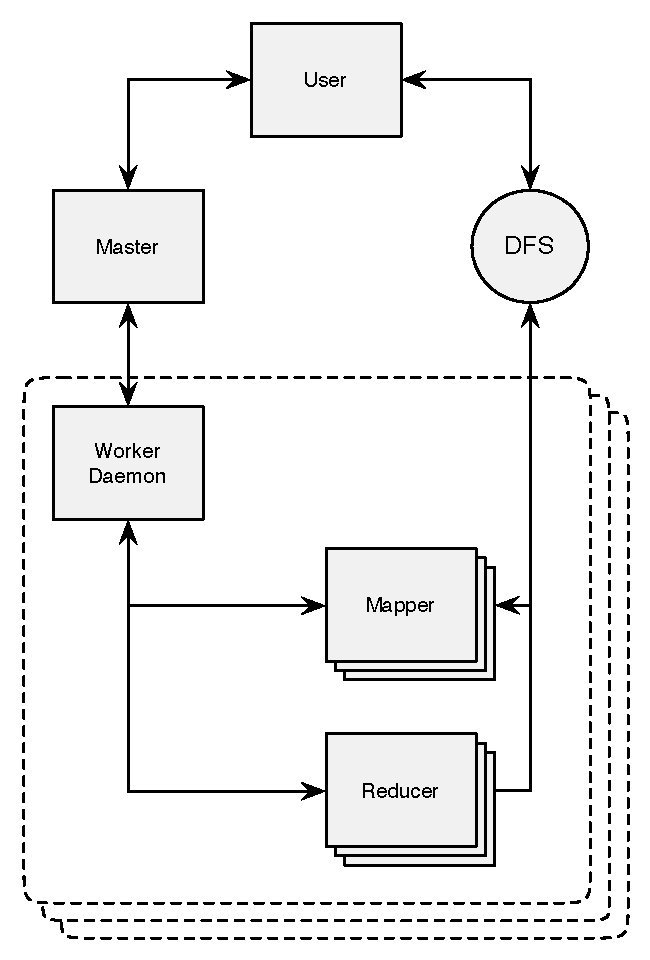
\includegraphics{Architecture.pdf}
}
\caption{The major components found in our architecture.}
\label{fig:arch}
\end{center}
\end{figure}


Our proposed architecture is shown in Figure~\ref{fig:arch}. We first describe the major difference between our proposed architecture and the architecture suggested in prior implementations of MapReduce. We then explain our architecture and the RPCs it uses to communicate by taking the reader through the running of a typical MapReduce job. We finish this section by describing our mechanisms for tolerating faults and summarize the RPCs used in our architecture.

\subsection{Main difference}

There are two major differences between our implementation and standard MapReduce. The first is the introduction of a local manager process called the \emph{WorkDaemon} (WD) that manages a single node. The second difference is that we use the \emph{Accumulator-PartialHash} (APH) aggregation scheme, as described in \citet{yu2009distributed}.

\subsubsection{WorkDaemon}

The first major difference is the WD that sits on each node that mediates all communication between the master and the worker---including RPCing intermediate key/values to the reducers. This has some advantages and disadvantages.

There are three advantages to this approach. The first is that mapper threads can free system resources by closing immediately upon completion. This is especially important in systems where memory is scarce. This property has a secondary advantage: it entirely removes a failure case. Jobs no longer need to be rerun if mappers crash after completion since the daemon is responsible for all RPC with the reducers. Additionally, since worker communication is centralized by the WD we can reduce network overhead by batching messages.

The principle disadvantage of the WD approach is that the WD takes the node down when it crashes.  Essentially, a node is removed from the MapReduce pool if the WD crashes. However, since the WD is isolated from the user's code and data we expect this to be a somewhat rare event.

\subsubsection{Accumulator-PartialHash}

The second major difference is the adoption of the APH aggregation scheme. \citet{yu2009distributed} describes the original MapReduce approach as the \emph{FullSort} method: all the records are gathered in memory and sorted by intermediate key immediately following the map phase\footnote{If there are too many key-value pairs to store in memory then they are sorted externally.}. This method has two principle disadvantages: it may be memory intensive (unless we always sort externally in which case it is slow), and requires every key-value pair to be present in memory before sorting. 

 APH aggregation alleviates both these problems. APH essentially combines the sort phase with the initial reduction. Each reduction task has a hashtable that maps keys to partial aggregation objects (PAOs). These PAOs, intuitively, are some sufficient description of an incomplete aggregation such that:
\begin{itemize}
 \item a new key-value pair can be \emph{added} to the PAO to yield a new PAO (\emph{i.e.} $p^t = p^{t-1} + v^t$);
 \item two PAOs can be \emph{merged} to form a new PAO (\emph{i.e.} $p^s = p^q \oplus p^r$).
\end{itemize}
The user describes a reduction with an initialization function, addition function and merger function instead of a single reduce function. When a new object (either a value or a PAO) with a particular key is give to a reducers task, the task adds it to or merges it with the appropriate PAO in the hashtable.

This new formulation yields some immediate advantages: if the PAO grows less than linearly in the number of key-value pairs then the memory used by a collection of PAOs will be less than then memory used by the complete list of key-value pairs. Additionally, by evicting any PAO object that either 1) is too large or 2) has a hash-value with many collisions, then we can guarantee an upper bound on the memory footprint for a reducer task. (The \emph{eviction policy}---the policy that selects PAOs to write to disk---must balance between evicting early to save memory and evicting late to maximize data compression).  

A second advantage of this approach is that we can start reducers immediately after at least one mapper finishes. This eliminates time spend waiting for key-value pairs to gather. Finally, since we don't sort. APH aggregation only requires key equality tests, rather than order comparisons. This means the programmer can avoid having to define spurious ``greater-than'' notions.

This formulation also has some disadvantages. Chief among these, some users may have a MapReduce formulation for their problem that assumes that the key-value pairs are initially sorted and rely on this fact to process them in sequence. We are breaking this for our prototype and explicitly assuming that key $k_i$ may be processed entirely independently from the processing of key $k_j$. In a full-featured release version of this program we would likely want to provide the user with a way of insisting that the key-value pairs be sorted, but we will not initially include this feature.

We initially worried that the PAOs might also obfuscate errors. For example, in the original MapReduce paper, key-value pairs could be flagged as `bad' and skipped if multiple reduce or map tasks fail on them. While we can still mark a record that causes repeated problems when we try to add it to a PAO as `bad', it is less clear what should be done if merging PAOs fails. Scrapping work and rerunning the tasks that generated the PAO could solve the problem if there was some order-dependent error, but what do we do if we just can't seem to get some PAOs to merge?

We believe that  the original intent of the bad-records was primarily to guard against anomalous data, and not logic problems with the user code. We can still provide reliability in the face of anomalous data by recording the last key-value pair that was successfully added to a PAO in the initial reduce, and some robustness to logical errors by rerunning PAO calculations, but we will  pass any repeated merger errors to the user---such errors represents a serious logical problem that is likely independent from \emph{where} the task was run. Additionally, if we have consistent problems merging two user-defined objects, this casts serious doubt on the validity of the user's code.

We feel that our design decision to use APH aggregation is reasonable for a MapReduce implementation that is primarily intended for memory-constrained systems.

\subsection{Typical Use}

So how does a typical MapReduce job look on this system? The sequence is initiated by the user when he contacts the master process and submits a MapReduce job using the \rpc{SubmitJob} RPC, which the user will block on\footnote{This is the only synchronous RPC call that we will use.}. In the initial version of our system we will assume that there is a single well-known master that is always available and that failures of the master are catastrophic. The user provides, in this initial RPC, the location of programs that carry out the \emph{map} function, and the PAO operations (which replace the Reduce function in our implementation). The user will pass this code to our program by implementing known functions and dynamically linking their object files into our code.

After receiving the initial message the master requests that the WorkDaemon on each node start \emph{mapper} threads with a \rpc{StartMapper} call. The master will try to place \emph{map} jobs on nodes that already have a replicated copy of the appropriate split of the input data.  We assume in this phase of the work that the user has access to the complete cluster and that the current MapReduce job is the only job running on the system. Later iterations of our work will have to include interactions with a cluster resource manager. We also assume that the WDs are already running on the worker nodes.

The WD, upon receipt of a \emph{map} work request, spawns a new \emph{mapper} TBB task for each request it gets. Because the WD never delays or rejects any work request the master is completely responsible for work scheduling (it maintains a tentative queue for each WD). The \rpc{StartMapper} call includes a list of input chunks from the DFS. For now, we will assume that each chunk belongs to a single file and that we do not have to worry about the boundaries of multi-chunk files---\textit{e.g.} if a text document spans two chunks a word does not start in one block and end in another.

Upon completion of its job a mapper immediately starts a mapper-level \emph{initial reduce}. The \emph{initial reducer} maintains a hashtable of PAOs, one for each key, and writes the resulting PAOs to local disk either when they are done or when they are evicted. The \emph{initial reducer} informs the WD when it is done, and the the WD contacts the master with a \rpc{ReportWorkComplete} to inform the master that it has some finished work. We will send all the completed PAOs for a reducer task as a single communication because this makes failure handling easier. In the future we may also have a node-level reducer that takes the PAOs from several map jobs and combines them into the same partition file.

In response to a \rpc{ReportWorkComplete} report the master may initiate some new \emph{final reducer} threads with \rpc{StartReducer}. Whenever a WD informs the master that it has some new PAOs to read, the master passes this information on to the appropriate \emph{final reducers} with an \rpc{ReportNewWork} call. If the PAOs  are local then the \emph{final reducer} can read them right from disk. If not, then the key/values are requested directly from the remote WD with a \rpc{SendData} call. The \emph{final reducer} starts executing the user's \emph{merge} code as soon as it has two PAOs.

While running the user's code the \emph{reducer} thread writes the final key-PAO pairs to a temporary local file. Upon completion the \emph{final reducer} writes this local file to the DFS and reports to the WD. The WD forwards this to the master by the \rpc{ReportWorkComplete} call.

\subsection{Fault Tolerance}
The above process needs to be resilient to machines and threads failing. We will tolerate worker nodes, worker tasks, and WorkDaemons crashing. We will not tolerate the master failing.

We use a `checking in' model to keep track of the dispatched jobs. This saves the master from having to actively query the status of each task. Whenever a mapper or a reducer task is working, the WD will periodically check its running status to ensure that it has not terminated before reporting that it has completed its work. Less frequently, the WD will send the master a list of jobs that terminated unexpectedly. On a node with all tasks reporting normally the list will be empty, but this message will still serve as a heartbeat.

If a job dies unexpectedly then the master will reschedule it: the master will send a \rpc{Kill} to the WD for that job and dispatch a new request for work. Notice that because the WD is responsible for sending data to the \emph{final reducers}, we do not need to notify any \emph{final reducers} about failed \emph{mappers}. 

If the entire node goes down (\textit{i.e.} the WD has not checked in for a while), then the master sends a \rpc{Kill} to the WD for all of its jobs, then \rpc{ReportFail}'s any reducer that are still waiting for PAOs from that node. Notice that since we ensure that all or no PAOs from a \emph{final reducer}, a node crash cannot leave us with a case where we have used some but not all of a \emph{initial reducer's} PAOs. Finally, the master reschedules all work on the downed node.

\subsection{RPC calls}

Here is a summary of the RPC calls used in our system:

\begin{table}[htdp]
\caption{Stored procedures on the master.}
\begin{center}
\begin{tabular}{|l|l|}\hline
\textbf{Procedure} & \textbf{Arguments}\\\hline
\rpc{SubmitJob} & R,M, Input Directory,\\
&\qquad  Output Directory\\
\rpc{CheckIn} & WorkerID, JobID List\\
\rpc{ReportWorkComplete} & WorkerID, JobID\\\hline
\end{tabular}
\end{center}
\label{tab:master_rpc}
\end{table}%

\begin{table}[htdp]
\caption{Stored procedures on the worker daemon}
\begin{center}
\begin{tabular}{|l|l|}\hline
\textbf{Procedure} & \textbf{Arguments}\\\hline
\rpc{StartMapper} & JobID, DFS chunk list \\
\rpc{StartReducer} & JobID, Key, OutputFile \\
\rpc{ReportNewWork} & Mapper IP, Mapper JobID\\
\rpc{ReportFail} & Mapper IP, Mapper JobID\\
\rpc{SendData} & JobID, Key\\
\rpc{Kill} & JobID\\\hline
\end{tabular}
\end{center}
\label{tab:worker_rpc}
\end{table}%



\section{Evaluation}
This section is the section subject to most future flucuation and should be
read as a preliminary or rough-draft version of our final evaluation section.

We plan on having two evaluation experiments, which may be composed of
several sub-experiments---this is unclear right now.  The first set of experiments
will run on $12$ machines located in the Satya server room.  These machines
will have Minnie configured on top of HDFS as well as Hadoop.  Benchmarks run
here will compare the two implementations of MapReduce on canoncial MapReduce
jobs.  This will give an understanding of the tradeoffs in using Minnie over a
more standard and established MapReduce implementation---Hadoop. The
second set of experiments will run on a FAWN cluster to demonstrate the
efficieny of the implementation in a low-memory environment.


\bibliographystyle{plainnat}
\bibliography{references}


\end{document}
